\documentclass[aps,prb,superscriptaddress,nofootinbib]{revtex4}
\usepackage{amsfonts}
\usepackage{amsmath}
\usepackage{amssymb}
\usepackage{graphbox}
\usepackage{graphicx}
\usepackage{caption}
\usepackage{bm}
\usepackage{bbm}
\usepackage{cancel}
\usepackage{color}
\usepackage{mathrsfs}
\usepackage[colorlinks,bookmarks=true,citecolor=blue,linkcolor=red,urlcolor=blue]{hyperref}
\usepackage{simpler-wick}
\usepackage{appendix}
\usepackage{float}
\usepackage{array}
\usepackage{booktabs}
\usepackage[export]{adjustbox}
\setlength{\parindent}{10 pt}
\setlength{\parskip}{2 pt}
\setcounter{MaxMatrixCols}{30}
\bibliographystyle{apsrev}
\newcommand{\RNum}[1]{\uppercase\expandafter{\romannumeral #1\relax}}
\newcommand{\normord}[1]{{:\mathrel{#1}:}}
\def\tbs{\textbackslash}
\def \tr{\operatorname{tr}}
\def \Tr{\operatorname{Tr}}


\begin{document}
\title{Nonlinear Sigma Model}
\author{Jie Ren}


\maketitle

In the context of spontaneous breaking of continuous symmetries, the nonlinear sigma model (NL$\sigma$M) arises as the effective description of the low energy physics.

\tableofcontents

\section{Effective Field Theory for Spontaneous Symmetry Breaking}

\subsection{U(1) Symmetry Breaking}
Consider the complex $\phi^4$ theory with negative mass term:
\begin{equation}
	\mathcal L = \partial^\mu \phi^* \partial_\mu \phi + m^2\phi^* \phi - \frac{g}{4}(\phi^*\phi)^2.
\end{equation}
The minimal energy field configuration is $|\phi_0|^2 = 2m^2/g$.
The field can be parameterized as
\begin{equation}
	\phi(x)=\left[\sqrt{\frac{2 m^{2}}{g}}+\frac{\sigma(x)}{\sqrt{2}} \right] \exp\left[{i \frac{\pi(x)}{F_{\pi}}}\right],
\end{equation}
with $F_{\pi}$ a real number.
After expanding the field around the minimal configuration, the effective Lagrangian is
\begin{equation}
	\mathcal{L}= \frac{1}{\lambda} \left[1+\frac{\sqrt{g}}{2m} \sigma(x) \right]^{2} \left(\partial_{\mu} \pi\right)^{2} +\frac{1}{2}\left(\partial_{\mu} \sigma\right)^{2}
	-\left(m^{2} \sigma^{2}+\frac{\sqrt{g} m}{2} \sigma^{3}+\frac{g}{16} \sigma^{4}\right)+\frac{m^{4}}{g},
\end{equation}
where $\lambda = gF_\pi^2/2m^2$.
This Lagrangian is called the Linear sigma model.
When $m\gg 1$, the $\sigma$ mode becomes infinitely massive and decoupled from the $\pi$ mode.
The Lagrangian is reduced to
\begin{equation}
	\mathcal L = \frac{1}{\lambda} (\partial_\mu \pi)^2 = \frac{1}{\lambda}\partial_\mu g \partial^\mu g^{-1},
\end{equation}
where $g \equiv e^{i\pi(x)} \in \mathrm{U}(1)$. 
Such model is the NL$\sigma$M on U(1) group.


\subsection{NL$\sigma$M on General Lie Groups}

We can generalize the idea of U(1)-symmetry breaking to arbitrary Lie group.
If a field theory under goes a $G$-symmetry breaking, and the fluctuation around the classical minimum is small (corresponding to the $m\rightarrow\infty$ limit in the U(1) case), then the low energy effective theory is described by the fluctuation on the $G$-manifold.
The most relevant action is 
\begin{equation}
	\mathcal L = \frac{1}{\lambda} \tr\left[\partial_\mu g \partial_\mu g^{-1}\right].
\end{equation}
Note that we define the field theory on $d$-dimensional Euclidean space, and we keep the coupling constant $\lambda$ unfixed.
The Lie group element $g$ is dimensionless, so that $[\lambda] = [d-2]$.

One noticeable difference of the path integral formalism is that the matrix field lives on the compact Lie group manifold.
The partition function is
\begin{equation}
	Z = \int D[g] e^{-S[g]},
\end{equation}
where $D[g]=\prod_x \int dg$ is the Haar measure of the Lie group, satisfying the conditions:
\begin{equation}
	\int dg = 1,\quad
	\int dg\ f(g) = \int dg\ f(h^{-1} g) = \int dg\ f(gh^{-1}).
\end{equation}
For simple Lie group, an element $g$ can be parametrized as
\begin{equation}
	g = \exp\left(i\sum_a \pi^a T^a\right),
\end{equation}
where the generators $\{T^a\}$ generate the Lie algebra of the Lie group.
Using this, we can formally expresses the theory in terms of $\pi$ field:
\begin{equation}
	\mathcal L = \frac{\tr[T^a T^b]}{\lambda}\partial_\mu\pi^a \partial_\mu \pi^b.
\end{equation}
Note that although the $\pi$ field, although quadratic, is not free, since it is defined on a nontrivial group manifold.
In general, we can express the Haar measure as
\begin{equation}
	dg = J(\pi) dp,
\end{equation}
where $J(\pi)$ is a function acting like a Jacobian. 
Note that in the vicinity of the identity, Jacobian is
\begin{equation}
	J(\pi) = 1 +O(\pi^4).
\end{equation}
Therefore, when we are studying the low energy property, the $\pi$ mode is nearly free.



\subsection{NL$\sigma$M on Coset Spaces}
\label{NLSM-coset}
Consider the situation where the symmetry of a model is broken from a large compact group $G$ down to some subgroup $H$.
The effective theory for the goldstone modes $g \in G/H$ is a NL$\sigma$M.
One way to represent the element $g \in G/H$ is to first choose an element $\Lambda\in G$ that commutes with all $h\in H$, i.e., $h\Lambda h^{-1}=\Lambda$.
The set
\begin{equation}
	\{Q(g) = g\Lambda g^{-1}|g\in G\}
\end{equation} 
is isomorphic to the coset space $G/H$.
As for the effective action, the symmetry principle requires (i) the action should be invariant under \textit{global} transformation of $G$: 
\begin{equation}
	S[g] = S[\tilde g g],\quad g\in G,
\end{equation}
and (ii) the action is invariant under local trnasformation of $H$:
\begin{equation}
	S[g] = S[gh], \quad h(x) \in H.
\end{equation}
The most relevant action satisfying (i) and (ii) is
\begin{equation}
	S[Q] = \frac{1}{\lambda}\int d^d x \tr[\partial^\mu Q \partial_\mu Q].
\end{equation}
In the exponential form of $g=e^{iW}$, note that we can use the subalgebra $\mathfrak{g}/\mathfrak{h}$ since the $\mathfrak h$-generated element is trivial.


\section{Effective Field Theory for Disordered Electrons}

Consider the non-relativistic electron gas under disordered potential:
\begin{equation}
	\mathcal L = \bar\psi \left[\partial_\tau -\frac{\nabla^2}{2m}-\mu+V(x) \right]\psi. 
\end{equation}
The potential is assumed to be independent Gaussian random variable at each $x$:
\begin{equation}
	P[V(x)] = \frac{1}{\sqrt{2\pi \gamma^2}}\exp\left[-\frac{V^2(x)}{2\gamma^2}\right].
\end{equation}
In the following, we are going to map the disordered system to a homogeneous one with multiple copies (replica).
We will then investigate the RG-flow of the effective action.

\subsection{Replica Trick}

The physical observable is those expectation value with disorder average:
\begin{equation}
	\langle O[\bar\psi,\psi] \rangle_{\mathrm{dis}} \simeq \left\langle \frac{\int D[\bar\psi,\psi] O\left[\frac{\delta}{\delta\bar J},\frac{\delta}{\delta J}\right] e^{-S[\bar\psi,\psi,V]+\psi J + \bar J \psi}}{\int D[\bar\psi,\psi] e^{-S[\bar\psi,\psi,V]+\psi J + \bar J \psi}}\right\rangle_\mathrm{dis}.
\end{equation}
As usual, we can define a generating function $Z[\bar J, J] \equiv \int D[\bar\psi,\psi] e^{-S[\bar\psi,\psi,V]+\psi J + \bar J \psi}$.
The expectation value is $\langle O\rangle_\mathrm{dis} = O\left[\delta_{\bar J},\delta _J \right] \langle \ln Z[\bar J, J] \rangle_\mathrm{dis}$.
The averaging involves $ln$, which is nonlinear and thus hard to calculate.
The replica trick use the fact
\begin{equation}
	\ln Z = \lim_{R\rightarrow 0}\frac{1}{R}(Z^R-1)
\end{equation}
to map the problem to an $R$-replicated system.
Correspondingly, we assign an internal index $a=1,\cdots,R$ to the fermion field $\psi$.
The total partition function can be expressed as
\begin{equation}
	Z = \int D[V] e^{-\frac{1}{2\gamma^2}\int d^d x V^2(x)} \int D[\bar\psi,\psi] e^{-\sum_{a=1}^R\int d^d x \bar\psi^a[\partial_\tau-\hat H + V(x)]\psi^a} 
	= \int D[\bar\psi,\psi] e^{-S_0-S_{\mathrm{dis}}}, 
\end{equation}
where $S_0$ is the free part and the disorder part becomes replica interaction when integrate out $V$:
\begin{equation}
	S_\mathrm{dis} = - \frac{\gamma^2}{2} \sum_{ab}\int d\tau_1d\tau_2 \int d^d x\ \bar\psi^a(x,\tau_1)\psi^a(x,\tau_1)\bar\psi^b(x,\tau_2)\psi^b(x,\tau_2).
\end{equation}
where $\gamma$ is the strength of the disorder.
For the electron propagator, the most relevant diagram is the rainbow diagrams, satisfying the self-consistent condition:

\begin{equation}
\begin{aligned}
	\Sigma(\omega,\bm p) &= 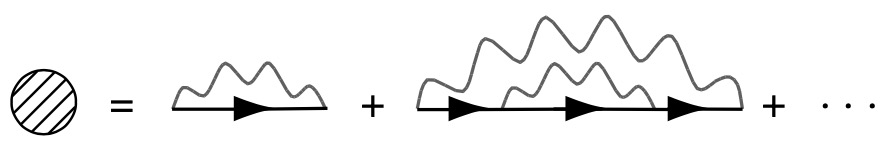
\includegraphics[vsmash=c,vshift=0.23cm,width=0.4\linewidth]{pics/rainbow.jpg} 
	= -\gamma^2 \int \frac{d^d q}{(2\pi)^d} G(\omega,\bm q) \\
	&= -\gamma^2 \int \frac{d^d q}{(2\pi)^d} \frac{1}{i\omega-\frac{\bm q^2}{2m}+\mu+\Sigma(\omega,\bm q)} 
	\simeq -\gamma^2 \int d\epsilon \frac{\nu(\epsilon)}{i\omega-\epsilon+\mu+\Sigma(\omega,\bm q)}
\end{aligned}
\end{equation}
The self-consistent condition can be solves with the ansatz
\begin{equation}\label{eq:al-self-energy}
	\Sigma(\omega,\bm p) = \frac{i}{2\tau} \operatorname{sign}\omega_n.
\end{equation}
When the imaginary part is relatively small, we have
\begin{equation}
	-\gamma^2 \int d\epsilon \frac{\nu(\epsilon)}{\mu-\epsilon+i(\omega+\frac{1}{2\tau}\operatorname{sign}\omega)}
	\simeq -\gamma^2 \mathcal P \int d\epsilon \frac{\nu(\epsilon)}{\mu-\epsilon}+i\pi\gamma^2\nu \operatorname{sign}\omega,
\end{equation}
where $\mathcal P$ is the principal value integral (which gives zero for the odd function), and $\nu$ is the density of states near the Fermi surface.
Therefore, $\tau^{-1}=2\pi\nu\gamma^2$.
The $\tau^{-1}$ has the physical meaning of scattering rate.


\subsection{Mean-Field Theory}

Now we consider the mean field theory of the interacting replica system.
When trying to decouple the vertex, we should notice from Eq.~(\ref{eq:al-self-energy}) that the pole of the propagator is non-analytic between $\omega>0$ and $\omega<0$.
In this way, the scattering $\psi^+ \psi^+ \rightarrow \psi^+\psi^+$ and $\psi^+ \psi^- \rightarrow \psi^+\psi^-$ should be considered separately. 
Luckily, for the system with time-reversal symmetry, we can treat those two channels on the same footing, we introduce a new ``time-reversal space" and define:
\begin{equation}
	\Psi(\tau)\equiv\begin{bmatrix}
		\psi(\tau) \\ \bar\psi^T(-\tau) 
	\end{bmatrix},\quad
	\bar\Psi(\tau) \equiv \begin{bmatrix}
		\bar\psi(\tau), & - \psi^T(-\tau)
	\end{bmatrix}.
\end{equation}
We note that the free action can be expressed in a simple form of $\Psi$ field:
\begin{equation}
\begin{aligned}
	S_0 &= -\int d^d x\ \bar\psi \hat G^{-1}\psi 
	= -\frac{1}{2}\int d^d x \left[\bar\psi \hat G^{-1}\psi + (\bar\psi \hat G^{-1}\psi)^T\right] \\
	&= -\frac{1}{2} \int d^d x \left[\bar\psi(\tau) \hat G^{-1}\psi(\tau) - \psi^T(\tau) \left. \hat G^{-1}\right|_{\partial\tau \rightarrow -\partial_\tau} \bar\psi^T(\tau)\right] \\
	&=-\frac{1}{2}\int d^d x \left[\bar\psi(\tau) \hat G^{-1}\psi(\tau) - \psi^T(-\tau) \hat G^{-1} \bar\psi^T(-\tau)\right] \\
	&= -\frac{1}{2}\int d^d x\ \bar\Psi(\tau) \hat G^{-1} \Psi(\tau).
\end{aligned}
\end{equation}
Note that we have put the frequency degrees of freedom into the vector form of $\Psi$ so the time integral/frequency summation is implicit in the vector inner product.
If we consider a cutoff with $2M$ frequencies of interest, $\Psi$ is then a $4MR$-dimensional vector.
The interacting action in terms of $\Psi$ field is:
\begin{equation}
	S_\mathrm{dis} = - \frac{\gamma^2}{8} \int d^d x\ (\bar\Psi\Psi)(x) (\bar\Psi\Psi)(x).
\end{equation}
We can then decouple the vertex using the Hubbard-Stratonovich transformation.




\subsection{Effective NL$\sigma$M}

Note that the disordered action can be expressed as a Gaussian integral:
\begin{equation}
	e^{-S_{\mathrm{dis}}[\bar\psi,\psi]} 
	= \int D[\Phi] e^{-S_1[\bar\psi,\psi,\Phi]} 
	= \int D[\Phi] \exp\left[-\frac{1}{2} \int d^d x \left(\tr \Phi^2 -i\frac{\gamma}{2}\bar\Psi\Phi\Psi \right)\right].
\end{equation}
The disorder-averaged partition function is then:
\begin{equation}
\begin{aligned}
	\langle Z \rangle_{\mathrm{dis}} &= \int D[\Phi] \int D[\bar\psi,\psi] \exp\left[-\frac{1}{2} \int d^d x \tr \Phi^2 -\frac{1}{2}\int d^d x \bar\Psi\left(-i\hat\omega-\frac{\nabla^2}{2m}-\mu -i\frac{\gamma}{2}\Phi\right)\Psi\right] \\
	&= \int D[\Phi] \exp\left[-\frac{1}{2}\int d^d x \tr \Phi^2 +\frac{1}{2}\tr\ln \hat G^{-1}[\Phi]\right].
\end{aligned}
\end{equation}
We assume for $\Phi$ is homogeneous in space, and the saddle-point condition $\delta S_{\mathrm{eff}}/\delta \Phi =0$ is
\begin{equation}
	\Phi = i \int d\epsilon \frac{\nu(\epsilon)}{i\omega -\epsilon+\mu+i\frac{\gamma}{2}\Phi}
	\simeq \pi\nu\operatorname{sign}\omega.
\end{equation}
In the replica space, we can write down the solution as $\bar \Phi = (\pi\nu)^{-1} \sigma_3$.
The general solution can be expressed as
\begin{equation}
	Q = T(\sigma_3\otimes \mathbb I) T^{-1},\quad T\in \mathrm{Sp}(4MR),
\end{equation}
where we note that (i) the matrix $\sigma_3$ is defined on the frequency degrees of freedom, and (ii) $T$ belong to Symplectic group since it should preserve the time-reversal symmetry.
That is, as the field $Q$ transforms as $Q(\tau_1-\tau_2) \sim \Psi(\tau_1) \bar\Psi(\tau_2)$.
Using the symmetry 
\begin{equation}
	\Psi^T(\tau)=-\bar\Psi(-\tau)(i\sigma_2^\mathrm{tr}),\quad
	\bar\Psi^T(\tau)=(i\sigma_2^\mathrm{tr})\Psi(-\tau),
\end{equation}
we know that $Q$ satisfies the symmetry condition:
\begin{equation}
	Q^T(\tau_1-\tau_2) = -(i\sigma_2^\mathrm{tr})\Psi(-\tau_2)\bar\Psi(-\tau_1)(i\sigma_2^\mathrm{tr})
	=\sigma_2^\mathrm{tr}Q(\tau_1-\tau_2)\sigma_2^\mathrm{tr}
\end{equation}
Also we note the subgroup $\mathrm{Sp}(2MR)\times\mathrm{Sp}(2MR)$ is invariant. 
Therefore $Q$ represent the coset space 
\begin{equation}
	G/H = \mathrm{Sp}(4MR)/\mathrm{Sp}(2MR)\times\mathrm{Sp}(2MR).
\end{equation}
We can then directly write down the effective action from the symmetry principle.
First, the fluctuation term is invariant under the $G$-symmetry.
The most relevant term is
\begin{equation}
	S_\mathrm{fl}[Q] = c_\mathrm{fl} \int d^d x \tr[\partial^\mu Q\partial_\mu Q].
\end{equation}
The most relevant term that explicitly break the $G$ symmetry to $H$ is
\begin{equation}
	S_{\omega}[Q] = c_\omega \int d^d x \tr[\hat \omega Q].
\end{equation}
The effective action is $S_\mathrm{eff}[Q] = S_\mathrm{fl}[Q]+S_{\omega}[Q]$.
When the frequency contribution to the action is negligible, the effective action is NL$\sigma$M:
\begin{equation}
	S_\mathrm{eff}[Q] = \int d^d x \tr[\partial^\mu Q \partial_\mu Q].
\end{equation}
Note that $Q$ can be parametrized as $Q=e^{iW} \Lambda e^{-iW}$, where the Lie algebra $W$ has the general form:\footnote{Note that $T$ is unitary and $W$ anti commute with $\Lambda=\sigma_3$.}
\begin{equation}\label{eq:AL-Liealg}
	W = \begin{pmatrix}
		0 & B \\ B^\dagger & 0
	\end{pmatrix}.
\end{equation}
The symmetry condition requires that
\begin{equation}
	\sigma_2^\mathrm{tr} e^{-iW^T} \Lambda e^{iW^T} \sigma_2^\mathrm{tr} 
	= e^{-i \sigma_2^\mathrm{tr} W^T \sigma_2^\mathrm{tr}} \Lambda e^{i \sigma_2^\mathrm{tr}W^T\sigma_2^\mathrm{tr}}
	= e^{iW} \Lambda e^{-iW},
\end{equation}
which implies $\sigma_2^\mathrm{tr}g\sigma_2^\mathrm{tr}=g^{-1}$, and also constraint the Lie algebra:
\begin{equation}
	\sigma_2^\mathrm{tr}W^T\sigma_2^\mathrm{tr} = -W \quad \Longrightarrow \quad
	\sigma_2^\mathrm{tr}B^T\sigma_2^\mathrm{tr} = -B^\dagger.
\end{equation}



\section{Renormalization Group of NL$\sigma$M on O($N$) Groups}

In this section, we discuss the renormalization group analysis of the O($N$)-NL$\sigma$M.
A canonical basis can be chosen for a simple Lie group.
The canonical basis $\{T^a\}$ for O($N$) group satisfies the following completeness relation:
\begin{equation}\label{eq:com-rel}
	\sum_{a} T_{i j}^{a} T_{k l}^{a} =\delta_{i l} \delta_{j k}-\delta_{i k} \delta_{j l}.
\end{equation} 
In addition, the trace of Lie algebra satisfies the orthogonal relation:
\begin{equation}
	\tr\left(T^{a} T^{b}\right)=\delta^{a b}.
\end{equation}
In the following, we carry out standard RG analysis for the O($N$)-NL$\sigma$M.



\subsection{Field Decomposition}
As usual, the matrix field $g$ can also be split into slow and fast components:
\begin{equation}
	g(r) = g_{\mathrm{s}}(r) g_{\mathrm{f}}(r).
\end{equation}
The action can be decomposed into three parts:
\begin{equation}
\begin{aligned}
	S[g] &= \frac{1}{\lambda}\int d^d x \tr[(\partial_\mu g_{\mathrm{s}} g_{\mathrm{f}} + g_{\mathrm{s}} \partial_\mu g_{\mathrm{f}})(\partial_\mu g_{\mathrm{f}}^{-1} g_{\mathrm{s}}^{-1}+g_{\mathrm{f}}^{-1}\partial_\mu g_{\mathrm{s}}^{-1})] \\
	&= \frac{1}{\lambda}\int d^d x\left( \tr[\partial_\mu g_{\mathrm{s}} \partial_\mu g_{\mathrm{s}}^{-1}]+\tr[\partial_\mu g_{\mathrm{s}} \partial_\mu g_{\mathrm{s}}^{-1}]+\tr[g_{\mathrm{s}}^{-1}\partial_\mu g_{\mathrm{s}} g_{\mathrm{f}} \partial_\mu g_{\mathrm{f}}^{-1}+\partial_\mu g_{\mathrm{s}}^{-1} g_{\mathrm{s}} \partial_\mu g_{\mathrm{f}} g_{\mathrm{f}}^{-1}] \right) \\
	&= S[g_{\mathrm{s}}] + S[g_{\mathrm{f}}] + S[g_{\mathrm{s}},g_{\mathrm{f}}].
\end{aligned}
\end{equation}
The actions for slow and fast field have the same form as the original one, and the coupling between the fast and the slow field is
\begin{equation}
\begin{aligned}
	S[g_{\mathrm{s}},g_{\mathrm{f}}] 
	&= \frac{1}{\lambda}\int d^d x \tr[g_{\mathrm{s}}^{-1}\partial_\mu g_{\mathrm{s}} g_{\mathrm{f}} \partial_\mu g_{\mathrm{f}}^{-1}+\partial_\mu g_{\mathrm{s}}^{-1} g_{\mathrm{s}} \partial_\mu g_{\mathrm{f}} g_{\mathrm{f}}^{-1}] \\
	&= \frac{2}{\lambda} \int d^d x\ \tr\left[g_{\mathrm{s}}^{-1}\partial_\mu g_{\mathrm{s}} \cdot g_{\mathrm{f}} \partial^\mu g_{\mathrm{f}}^{-1}\right].
\end{aligned}
\end{equation}
As usual, the coarse-graining correspond to integrating out the fast field.
To the second order, the result is
\begin{equation}
	S_{\mathrm{eff}}[g_{\mathrm{s}}] 
	= S[g_{\mathrm{s}}] + \langle S[g_{\mathrm{s}},g_{\mathrm{f}}]\rangle_{\mathrm{f}}-\frac{1}{2}\langle S[g_{\mathrm{s}},g_{\mathrm{f}}]^2\rangle^c_{\mathrm{f}}.
\end{equation}
Consider the first order perturbation, where we should evaluate $\langle g_{\mathrm{f}} \partial^\mu g_{\mathrm{f}}^{-1}\rangle_{\mathrm{f}}$, which is zero because of the rotational symmetry.
For the second order, in evaluating the $\langle\cdots\rangle_\mathrm{f}$, we approximate the fast field as free field:
\begin{equation}
	S[g_{\mathrm{f}}] = \frac{1}{\lambda} \int d^d x \partial_\mu \pi^a \partial^\mu \pi^b \tr[T^a T^b]
	= \frac{1}{2}\int \frac{d^d p}{(2\pi)^d} \pi^a_pG^{-1}_p\pi^a_{-p},
\end{equation}
where the propagator of the $\pi$ field is
\begin{equation}
	G_p = \frac{\lambda}{2 p^2}.
\end{equation}
The energy-shell integral can then be carried out.



\subsection{Energy-Shell Integral}
We are going to express the field theory in terms of the Lie algebra.
To simplify the notation, we define 
\begin{equation}
	g_{\mathrm{f}} = e^{iW} = 1 + i W - \frac{1}{2}W^2 + O(W^3).
\end{equation}
To the second order of $\pi$, the interacting action to the second order of $\pi$ is
\begin{equation}
\begin{aligned}
	S[g_{\mathrm{s}},g_{\mathrm{f}}] 
	&= \frac{2}{\lambda} \int d^d x\ \tr\left[g_{\mathrm{s}}^{-1}\partial^\mu g_{\mathrm{s}} \cdot \left(1+iW-\frac{1}{2}W^2\right) \partial_\mu \left(1-iW-\frac{1}{2}W^2\right)\right] +O(W^3)\\
	&= \frac{1}{\lambda} \int d^d x\ \tr\left(g_{\mathrm{s}}^{-1}\partial^\mu g_{\mathrm{s}} \cdot [W,\partial_\mu W]\right)+O(W^3) \\
	&= \frac{2i}{\lambda}\int_{d\Lambda} \frac{d^d p}{(2\pi)^d}\int\frac{dq}{(2\pi)^d} p^\mu \tr\left[\Phi_{\mu,-q}W_{p+q}W_{-p}\right]+O(W^3),
\end{aligned}
\end{equation}
where we have defined $\Phi_\mu = g_{\mathrm{s}}^{-1}\partial_\mu g_{\mathrm{s}}$.
Note that in the expansion, there is actually a linear term $\partial_\mu W$, which vanish upon integral due to the rotational symmetry.
To the second order,
\begin{equation}
	\frac{1}{2}\langle S[g_{\mathrm{s}},g_{\mathrm{f}}]^2\rangle_{\mathrm{f}}^c
	= \frac{2}{\lambda^2} \int_{d\Lambda}\frac{d^d p}{(2\pi)^d} \frac{d^d p'}{(2\pi)^d}\int\frac{d^d q}{(2\pi)^d}\frac{d^d q'}{(2\pi)^d} p^\mu p^{\prime\nu} 
	\langle \tr\left[\Phi_{\mu,-q}W_{p+q}W_{-p}\right]\tr\left[\Phi_{\nu,-q'}W_{p'+q'}W_{-p'}\right]\rangle^c_{\mathrm{f}}.
\end{equation}
The next step is to evaluate the expectation value,
\begin{equation}
	\langle \tr\left[\Phi_{\mu,-q}W_{p+q}W_{-p}\right]\tr\left[\Phi_{\nu,-q'}W_{p'+q'}W_{-p'}\right]\rangle^c_{\mathrm{f}}
	=  \tr\left[\Phi_{\mu,-q}T^aT^b\right]\tr\left[\Phi_{\nu,-q'}T^c T^d\right]\langle\pi^a_{p+q}\pi^b_{-p}\pi^c_{p'+q'}\pi^d_{-p'}\rangle^c_{\mathrm{f}}.
\end{equation}
The connected 4-point function for free $\pi$ field is
\begin{equation}
\begin{aligned}
	\langle\pi^a_{p+q}\pi^b_{-p}\pi^c_{p'+q'}\pi^d_{-p'}\rangle^c_{\mathrm{f}}
	&= \left[\delta_{ac}\delta_{bd}\delta(q+q')\delta(p+p') + \delta_{ad}\delta_{bc}\delta(p-p'+q)\delta(p'-p+q')\right]\frac{\lambda^2}{4p^2(p+q)^2} \\
	&\simeq [\delta_{ac}\delta_{bd}\delta(p+p')+\delta_{ad}\delta_{bc}\delta(p-p')]\delta(q+q')\frac{\lambda^2}{4p^4}.
\end{aligned}
\end{equation}
From this we have
\begin{equation}
\begin{aligned}
	\langle \cdots \rangle^c_{\mathrm{f}}
	= (\Phi_{\mu,-q})_{ij} (\Phi_{\nu,q})_{lm} \left[T_{jk}^a T_{mn}^a T_{ki}^b T_{nl}^b \delta(p+p') +T_{jk}^a T_{nl}^a T_{ki}^b T_{mn}^b \delta(p-p')\right] \delta(q+q')\frac{\lambda^2}{4p^4}.
\end{aligned}
\end{equation}
Now using the completeness relation in Eq.~(\ref{eq:com-rel}), and note the fact
\begin{equation}
\begin{aligned}
	A_{ij}B_{lm}(\delta_{jn}\delta_{km}-\delta_{jm}\delta_{kn})(\delta_{kl}\delta_{in}-\delta_{kn}\delta_{il})
	&= A_{ii}B_{ll} - A_{ij}B_{ij} - A_{ij}B_{ij}+A_{ij}B_{ij}\delta_{kk}, \\
	A_{ij}B_{lm}(\delta_{jl}\delta_{kn}-\delta_{jn}\delta_{kl})(\delta_{kn}\delta_{im}-\delta_{km}\delta_{in})
	&= A_{ij}B_{ji}\delta_{kk} - A_{ij}B_{ji}-A_{ij}B_{ji}+A_{ii}B_{jj}.
\end{aligned}
\end{equation}
Note that the Lie algebra basis $\{T^a\}$ is anti-symmetric for O($N$) groups. 
That means
\begin{equation}
	\left(g_{\mathrm{s}}^{-1}\partial_\mu g_{\mathrm{s}}\right)^T = \partial_\mu g_{\mathrm{s}}^T g_{\mathrm{s}}^{-T}
	=\partial_\mu g_{\mathrm{s}}^{-1} g_{\mathrm{s}} 
	\simeq -g_{\mathrm{s}}^{-1} \partial_\mu g_{\mathrm{s}}.
\end{equation}
Therefore,
\begin{equation}
\begin{aligned}
	\frac{1}{2}\langle S[g_{\mathrm{s}},g_{\mathrm{f}}]^2\rangle_{\mathrm{f}}^c
	&\simeq \frac{1}{2} \int \frac{d^d p}{(2\pi)^d}  \frac{p^\mu p^\nu}{p^4} 2(N-2) \int \frac{d^d q}{(2\pi)^d} \tr[\Phi_{\mu,q}\Phi_{\nu,-q}] \\
	&= \frac{N-2}{d}\int \frac{d^d p}{(2\pi)^d}  \frac{1}{p^2} \int d^d x\ \tr[\partial^\mu g_{\mathrm{s}} \partial_\mu g_{\mathrm{s}}^{-1}] \\
	&= C(d,N) \int d^d x\ \tr[\partial^\mu g_{\mathrm{s}} \partial_\mu g_{\mathrm{s}}^{-1}]
\end{aligned}
\end{equation}
Indeed, the second order perturbation produce the action of the same form as the original one, with coefficient
\begin{equation}
	C(d,N) = \frac{N-2}{d}\int \frac{d^d p}{(2\pi)^d}  \frac{1}{p^2}.
\end{equation}



\subsection{Beta Function and RG-Flow}

The critical dimension for NL$\sigma$M is 2, we set $d=2+\varepsilon$,
\begin{equation}
	C(d,N) 
	= \frac{(N-2)\Omega_2}{2(2\pi)^2}\int^1_{b^{-1}} \frac{dp}{p}+ O(\varepsilon)
	= \frac{(N-2)\ln s}{4\pi} + O(\varepsilon).
\end{equation}
After the rescaling $k\rightarrow k'=sk$, the coefficient becomes:
\begin{equation}
	\lambda' = \left[1-\frac{(N-2)\ln s}{4\pi}\lambda\right]^{-1} s^{-\epsilon} \lambda
	= \lambda + \ln s \left[\frac{(N-2)}{4\pi}-\epsilon\right]\lambda.
\end{equation}
Let $s = e^{dl}$, the beta function is
\begin{equation}
	\beta(\lambda) \equiv \frac{d \ln \lambda}{dl} = \frac{(N-2)\lambda}{4\pi}-\epsilon.
\end{equation}
The RG-flow of the coupling is:
\begin{equation*}
	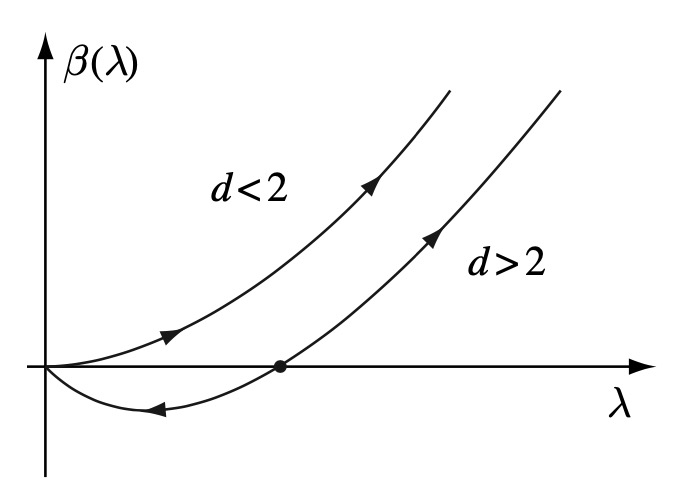
\includegraphics[width=0.3\linewidth]{pics/RG-flow.jpg}
\end{equation*}
From the beta function, we know at low dimension $d < 2$, $\beta(\lambda) > 0$.
In the low-energy limit, $1/\lambda \rightarrow 0$, i.e., the NL$\sigma$M would have little energy cost to create $\pi$ excitation.
The system is thus in the disordered phase.
On the other hand, for $d>0$, there is order-disorder transition at 
\begin{equation*}
	\lambda_* = \frac{4\pi(d-2)}{N-2}.
\end{equation*}
A special case is the O(2)-NL$\sigma$M at $d=2$, which requires additional analysis.



\section{BKT Phase Transition}

For the O(2) case, the NL$\sigma$M is described by an angle $\phi$:
\begin{equation}
	\mathcal L = \frac{1}{\lambda}(\partial_\mu\phi)^2 + g\cos(\phi),
\end{equation}
where we have introduced an external field for the later convenience.
We can renormalize $\theta$ so that the kinetic term is canonical:
\begin{equation}
	\mathcal L = \frac{1}{2}(\partial_\mu \phi)^2 + g\cos(\beta \phi),
\end{equation}
where $\beta=\sqrt{\lambda/2}$.
The external field term will be regarded as the perturbation, the running coupling $g$ will be computed by standard RG procedure.



\subsection{First Order Beta Function}
When write $\phi$ as the sum of slow and fast modes: $\phi=\phi_{\mathrm{s}}+\phi_{\mathrm{f}}$, the partition function is
\begin{equation}
	Z = \left\langle\exp\left\{-g \int d^2 x \cos\left[\beta(\phi_{\mathrm{s}}+\phi_{\mathrm{f}})\right] \right\}\right\rangle_{\mathrm{f}} \int D[\phi_{\mathrm{s}}] \exp\left[-\frac{1}{2}\int d^2x (\partial_\mu\phi_{\mathrm{s}})^2\right].
\end{equation}
We then consider the effective action to the second order:
\begin{equation}
	S_{\mathrm{eff}} = S_0 + \langle S_1\rangle_{\mathrm{f}} - \frac{1}{2}\langle S_1^2\rangle_{\mathrm{f}}^c
\end{equation}
where $S_0$ comes from the kinetic term and $S_1$ the perturbation.
To the first order,\footnote{Note the identity: $\cos\left[\beta(\phi_{\mathrm{s}}+\phi_{\mathrm{f}})\right]=\cos(\beta\phi_{\mathrm{s}})\cos(\beta\phi_{\mathrm{f}})-\sin(\beta\phi_{\mathrm{s}})\sin(\beta\phi_{\mathrm{f}})$. Note the fact that $\sin(\beta\phi_{\mathrm{f}})$ term will not contribute when integrated over the fast field.}
\begin{equation}
\begin{aligned}
	\langle S_1\rangle &= g \int d^2 x \left\langle\cos\left[\beta(\phi_{\mathrm{s}}+\phi_{\mathrm{f}})\right] \right\rangle_{\mathrm{f}} 
	= g \int d^2 x \cos(\beta\phi_{\mathrm{s}})\langle\cos(\beta\phi_{\mathrm{f}})\rangle_{\mathrm{f}}.
\end{aligned}
\end{equation}
We then compute the expectation over the fast field:\footnote{Note that fact $\langle \exp(i\beta\phi_{\mathrm{f}})\rangle = \exp(-\frac{1}{2}\beta^2 \langle\phi_{\mathrm{f}}^2\rangle)$.}
\begin{equation}
	\left\langle \cos(\beta\phi_{\mathrm{f}})\right\rangle_{\mathrm{f}}
	= \left\langle \frac{e^{i\beta\phi_{\mathrm{f}}} + e^{-i\beta\phi_{\mathrm{f}}}}{2}\right\rangle_{\mathrm{f}}
	= \exp\left({-\frac{1}{2}\beta^2\langle\phi_{\mathrm{f}}^2\rangle}\right) 
	= \exp\left[-\frac{\beta^2}{4\pi}\int_{d\Lambda}\frac{dk}{k} \right] 
	= s^{-\beta^2/4\pi}.
\end{equation}
The coarse-graining $x\rightarrow x'=s^{-1}x$ produce additional $s^{2}$ factor
In this way, the rescaling of $g$ is:
\begin{equation}
	g \rightarrow s^{2-\frac{\beta^2}{4\pi}} g.
\end{equation}
Let $s=e^{dl}$, the beta in the first order is
\begin{equation}
	\frac{d \ln g}{dl} = 2-\frac{\beta^2}{4\pi}.
\end{equation}


\subsection{Second Order Field Renormalization}
Now consider the second-order expansion
\begin{equation}
	\langle S_1^2\rangle_{\mathrm{f}}^c = \langle S_1^2\rangle_{\mathrm{f}} - \langle S_1^2\rangle_{\mathrm{f}}^2.
\end{equation}
The first term is (we denote $\phi(x_i)$ as $\phi_i$ for notational simplicity):
\begin{equation}
\begin{aligned}
	\langle S_1^2\rangle_{\mathrm{f}} &= g^2 \int d^2x_1 d^2x_2 \langle \cos(\beta\phi_1) 
		\cos(\beta \phi_2) \rangle_{\mathrm{f}} 
	= \frac{g^2}{2} \int d^2x_1 d^2x_2 \left\langle \cos\left[\beta(\phi_1+\phi_2)\right] + \cos\left[\beta(\phi_1-\phi_2)\right] \right\rangle_{\mathrm{f}} \\
	&= \frac{g^2}{2} \int d^2x_1 d^2x_2 \left\{\langle\cos\left[\beta(\phi_{\mathrm{f},1}+\phi_{\mathrm{f},2})\right]\rangle_{\mathrm{f}}\cos\left[\beta(\phi_{\mathrm{s},1}+\phi_{\mathrm{s},2})\right]  + 
	\langle\cos[\beta(\phi_{\mathrm{f},1}-\phi_{\mathrm{f},2})]\rangle_{\mathrm{f}}\cos\left[\beta(\phi_{\mathrm{s},1}-\phi_{\mathrm{s},2})\right]\right\}.
\end{aligned}
\end{equation}
Similarly, we have neglect all $\sin(\beta\phi_{\mathrm{f}})$ terms.
The averaging gives:
\begin{equation}
\begin{aligned}
	\langle S_1^2\rangle_{\mathrm{f}}
	= \frac{g^2}{2} \int d^2x_1 d^2x_2 \left\{e^{-\frac{\beta^2}{2}\langle[\phi_{\mathrm{f},1}+\phi_{\mathrm{f},2}]^2\rangle} \cos[\beta\phi_{\mathrm{s},1}+\beta\phi_{\mathrm{s},2}] + 
	  e^{-\frac{\beta^2}{2}\langle[\phi_{\mathrm{f},1}-\phi_{\mathrm{f},2}]^2\rangle} \cos[\beta\phi_{\mathrm{s},1}-\beta\phi_{\mathrm{s},2}] \right\}.
\end{aligned}
\end{equation}
For the second term,
\begin{equation}
\begin{aligned}
	\langle S_1\rangle_{\mathrm{f}}^2 &= \left[g\int d^2 x \left\langle \cos(\beta\phi_{\mathrm{s}}+\beta\phi_{\mathrm{f}})\right\rangle_{\mathrm{f}} \right]^2 
	= \left[g\int d^2 x \cos(\beta\phi_{\mathrm{s}}) \exp\left(-\frac{\beta^2}{2}\langle\phi_{\mathrm{f}}^2\rangle_{\mathrm{f}} \right)\right]^2 \\
	&= \frac{g^2}{2}e^{-\beta^2 \langle \phi_{\mathrm{f}}^2\rangle_{\mathrm{f}}} \int d^2x_2 d^2 x_2 \left\{ \cos[\beta(\phi_{\mathrm{s},1}+\phi_{\mathrm{s},2})] + \cos[\beta(\phi_{\mathrm{s},1}-\phi_{\mathrm{s},2})] \right\}
\end{aligned}
\end{equation}
The subtraction is
\begin{equation}
	S^{(2)}_{\mathrm{eff}}
	= g^2 e^{-\beta^2\langle\phi_{\mathrm{f}}^2\rangle} \int_{x_1,x_2}  \left\{
		\left(e^{-\beta^2 \langle\phi_{\mathrm{f},1}\phi_{\mathrm{f},2}\rangle}-1 \right)\cos\left[\beta(\phi_{\mathrm{s},1} +\phi_{\mathrm{s},2})\right] 
	 + \left(e^{\beta^2 \langle\phi_{\mathrm{f},1})\phi_{\mathrm{f},x})\rangle}-1 \right)\cos\left[\beta(\phi_{\mathrm{s},1} -\phi_{\mathrm{s},2})\right] \right\}.
\end{equation}
Formally, the first term gives the correction to the external field, while the second term appears to be additional.
We will show in the following that the second term actually correct the kinetic term.
Consider the bosonic correlation
\begin{equation}
	\mathcal G(\bm x) \equiv \langle \phi_{\mathrm{f}}(x) \phi_{\mathrm{f}}(0)\rangle_{\mathrm{f}} = F(\bm x) dl + O(dt^2).
\end{equation}
A straightforward calculation with the hard cut-off yields $F(\bm x)$ a Bessel function with long oscillating tail.
However, it can be shown that implementing a smooth cut-off will make $F(\bm x)$ short ranged.
For this reason, we can switch to the center-of-mass coordinate:
\begin{equation}
	\bm R = \frac{\bm x_1 + \bm x_2}{2}, \quad \bm r = \bm x_1 - \bm x_2.
\end{equation}
In this way, the term $\cos\left[\beta(\phi_{\mathrm{s},1}+\phi_{\mathrm{s},2})\right]$ is approximated by a $\cos\left[2\beta\phi_{\mathrm{s}}(x)\right]$ term, which is oscillating at double frequency, and thus is regarded as irrelevant.

The remaining term can be simplified by the approximation:
\begin{equation}
	\cos\left[\beta\phi_{\mathrm{s},1} -\beta\phi_{\mathrm{s},2}\right]
	\sim 1-\frac{\beta^2}{2} [\bm r \cdot \nabla\phi_{\mathrm{s}}(\bm R)]^2.
\end{equation}
The constant term only contributes to the the infinity of free energy.
The non-trivial contribution is:\footnote{Note that fact: $\int d^2r\ r_i r_j = \delta_{ij} \int r dr d\theta\ r^2 \cos^2(\theta) = \pi \delta_{ij} \int dr\ r^3$.}
\begin{equation}
\begin{aligned}
	&\ \int d^2 R \int d^2 r \left(e^{\beta^2 \langle\phi_{\mathrm{f},1}\phi_{\mathrm{f},2}\rangle}-1 \right)\cos\left[\beta(\phi_{\mathrm{s},1}-\phi_{\mathrm{s},2})\right] 
	\simeq -\frac{\beta^4}{2} \int d^2 R \int d^2r F(\bm r) [\bm r \cdot \nabla\phi_{\mathrm{s}}(\bm R)]^2 \\
	\simeq &\ -\frac{\pi \beta^4}{2} \left[\int_0^\infty dr\ r^3 F(r)\right]dl \int d^2 R [\nabla\phi_{\mathrm{s}}(\bm R)]^2 
	\equiv -\pi \beta^4 A dl \times \frac{1}{2}\int d^2 R [\nabla\phi(\bm R)]^2.
\end{aligned}
\end{equation}
We see the second order perturbation renormalize the free field, as it change normalization of the field:
\begin{equation}
	\phi \rightarrow \phi' = Z^{\frac{1}{2}} \phi, \quad 
	Z^{\frac{1}{2}} = 1 +\frac{g^2}{2} \pi \beta^4 A dl.
\end{equation}
To preserve the form of the $\cos(\beta\phi)$ term, we have to shift
\begin{equation}
	\beta \rightarrow \beta' = Z^{-\frac{1}{2}}\beta = \beta-\frac{1}{2}\pi g^2\beta^5 A dl.
\end{equation}
The RG-flow for $\beta$ is then
\begin{equation}
	\frac{d\beta}{dl} = -\frac{1}{2}\pi g^2\beta^5 A.
\end{equation}
Near the critical point ($g_* = 0$, $\beta_* = \sqrt{8\pi}$), we keep only lowest order term, the prefactor $e^{-\beta^2\langle\phi_{\mathrm{f}}^2\rangle}$ is then neglected, and we will not consider second order correction to external field here.
We introduce a new set of variables:
\begin{equation}
	x \equiv 2 - \frac{\beta^2}{4\pi}, \quad
	y \equiv 4\pi \sqrt{8\pi A} g.
\end{equation}
The RG-flow is then
\begin{equation}
	\frac{dx}{dl} = y^2, \quad
	\frac{dy}{dl} = xy.
\end{equation}
The flow diagram is
\begin{equation*}
	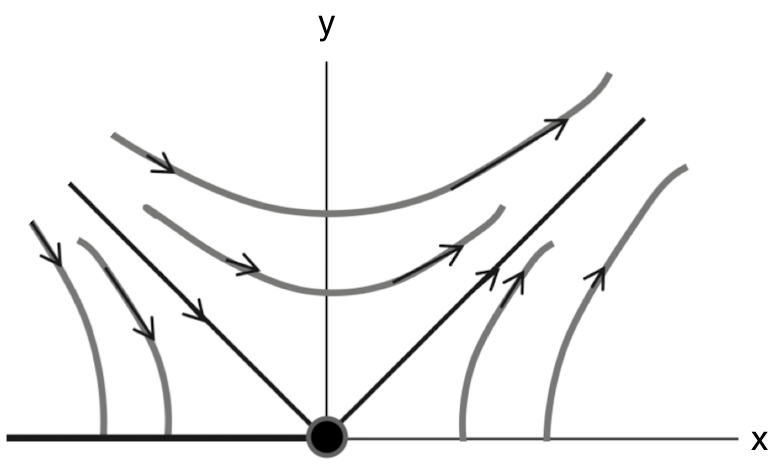
\includegraphics[width=0.3\linewidth]{pics/KT-RG-flow.png}
\end{equation*}
When $x+y<0$, the coupling will flow to $g=0$, corresponding to the KT phase; otherwise the coupling flows to $g\rightarrow\infty$ corresponding to the disordered phase.


\section{Renormalization Group for NL$\sigma$M on Coset Spaces}


\subsection{NL$\sigma$M on 2-Sphere}

We now consider the NL$\sigma$M on $\mathrm{SU}(2)/\mathrm{U}(1)$ space.
Such NL$\sigma$M gives the effective theory of the (classical) 3D ferromagnetic system.
It will turn out that the RG equation for the disordered electron is the same as the NL$\sigma$M on the 2-sphere.

For $(G,H)=(\mathrm{SU}(2),\mathrm{U}(1))$ case, the matrix field $Q$ can be represented as
\begin{equation}
	Q = g \sigma_3 g^{-1},\quad g \in \mathrm{SU}(2).
\end{equation}
We first decompose the field $g=g_{\mathrm{s}} g_{\mathrm{f}}$, the action can be written as
\begin{equation}
	S[g] = \frac{1}{\lambda}\int d^d x \tr[\partial^\mu (g_{\mathrm{s}} g_{\mathrm{f}} \sigma_3 g_{\mathrm{f}}^{-1} g_{\mathrm{s}}^{-1})\partial_\mu(g_{\mathrm{s}} g_{\mathrm{f}} \sigma_3 g_{\mathrm{f}}^{-1} g_{\mathrm{s}}^{-1})]
\end{equation}
Let $Q_{\mathrm{f}}\equiv g_{\mathrm{f}} \sigma_3 g_{\mathrm{f}}^{-1}$, the derivative term can be simplified to
\begin{equation}
	\tr[\partial_\mu(g_{\mathrm{s}} Q_{\mathrm{f}} g_{\mathrm{s}}^{-1})] = \tr[\partial_\mu Q_{\mathrm{f}} +[\Phi_\mu,Q_{\mathrm{f}}]],
\end{equation}
where $\Phi_\mu \equiv g_{\mathrm{s}}^{-1}\partial_\mu g_{\mathrm{s}}$.
Now consider the algebra $W=\mathfrak{su}(2)/\mathfrak{u}(1)$, which can be parametrized by an off-diagonal matrix with complex entries:
\begin{equation}
	W = \begin{pmatrix}
		0 & z \\ \bar z & 0
	\end{pmatrix}.
\end{equation}
Note that $W$ anti-commutes with $\sigma_3$, a straightforward expansion to the second order of $W$ gives:
\begin{equation}
	Q_{\mathrm{f}} = \sigma_3(1+2iW-2W^2)+O(W^3).
\end{equation}
Then, consider the term quadratic in $W$:
\begin{equation}\label{eq:AL-Seff}
\begin{aligned}
	S_{\mathrm{s}}[\Phi] &= \frac{1}{\lambda}\int d^d x \tr\left([\Phi_\mu,\sigma_3]^2\right) 
		= \frac{1}{\lambda}\int d^d x \tr[\partial^\mu Q\partial_\mu Q], \\
	S_{\mathrm{f}}[W] &= \frac{4}{\lambda}\int d^d x \tr[\partial^\mu W \partial_\mu W], \\
	S_{\mathrm{c}}[g_{\mathrm{s}},W] &= -\frac{8}{\lambda}\int d^d x \tr[\Phi_\mu W \sigma_3 \Phi_\mu W\sigma_3 + \Phi_\mu \sigma_3 \Phi_\mu \sigma_3 W^2].
\end{aligned}
\end{equation}
For the free theory, insert the parametrized form:
\begin{equation}
	S_{\mathrm{f}}[\bar z, z] =  \int \frac{d^d p}{(2\pi)^d} \frac{8\bm p^2}{\lambda} \bar{z}_{\bm{p}} z_{\bm{p}}.
\end{equation}
The propagator is $G(\bm p) = \lambda/8\bm p^2$. 
The coupling part of the action is
\begin{equation}
	S_{\mathrm{c}}\left[g_{\mathrm{s}}, z, \bar{z}\right]=-\frac{8}{\lambda} \int d^{d} x \operatorname{tr}\left(\Phi_{\mu}\left(z E_{12}-\bar{z} E_{21}\right) \Phi_{\mu}\left(z E_{12}-\bar{z} E_{21}\right)+\Phi_{\mu} \sigma_{3} \Phi_{\mu} \sigma_{3} z \bar{z}\right)
\end{equation}
The first-order correction to the effective action is $S_\mathrm{eff}[g_{\mathrm{s}}] = S[g_{\mathrm{s}}] + \langle S_{\mathrm{c}}[g_{\mathrm{s}},z,\bar z]\rangle_{\mathrm{f}}$.
For the slow field $\Phi_\mu$, note that we can shift the the variable $g_{\mathrm{s}} \rightarrow g_{\mathrm{s}} h$ which results in $\Phi_\mu \rightarrow \Phi_\mu + h^{-1}\partial_\mu h$.
We can always find a suitable local transformation such that $\Phi_\mu$ is off-diagonal.
In this way,
\begin{equation}
\begin{aligned}
	\langle S_{\mathrm{c}}[g_{\mathrm{s}},z,\bar z]\rangle_{\mathrm{f}} 
	&= -\frac{8}{\lambda} \int d^{d} x \operatorname{tr}\left[\Phi_{\mu} \sigma_{3} \Phi_{\mu} \sigma_{3} \right] \left\langle  \bar z z \right\rangle_{\mathrm{f}} 
	= -\frac{8}{\lambda} \int d^{d} x \operatorname{tr}\left[\Phi_{\mu} \sigma_{3} \Phi_{\mu} \sigma_{3} \right] \int_{d\Lambda} \frac{d^d p}{(2\pi)^d}\frac{\lambda}{8p^2} \\
	&= -\frac{I_2}{4} \int d^{d} x \operatorname{tr}\left([\Phi_{\mu},\sigma_{3}]^2\right).
\end{aligned}
\end{equation}
where we denote 
\begin{equation}
	I_n = \int_{d\Lambda} \frac{d^d p}{(2\pi)^d}\frac{1}{p^n}.
\end{equation}
Note that $\tr\left([\Phi_{\mu},\sigma_{3}]^2\right) = \tr[\partial^\mu Q_{\mathrm{s}} \partial_\mu Q_{\mathrm{s}}]$, which lead to the renormalization condition:
\begin{equation}
	\frac{1}{\lambda'} = s^{d-2}\left(\frac{1}{\lambda} -\frac{I_2}{4}\right).
\end{equation}
For the dimension $d=2+\varepsilon$, and let $s=e^{dl}$
\begin{equation}
	\lambda' = \lambda \left(1-\varepsilon dl + \frac{\lambda}{8\pi} dl \right).
\end{equation}
The beta function is
\begin{equation}
	\frac{d\lambda}{dl} = \frac{\lambda}{8\pi} - \varepsilon.
\end{equation}


\subsection{NL$\sigma$M on $\mathrm{Sp}(4MR)/\mathrm{Sp}(2MR)\times\mathrm{Sp}(2MR)$}

Now we turn to NL$\sigma$M on the coset space of $\mathrm{Sp}(4MR)/\mathrm{Sp}(2MR)\times\mathrm{Sp}(2MR)$.
The derivation till Eq.~(\ref{eq:AL-Seff}) still holds, with the slight modification that (i) $\sigma_3$ is now regarded as the matrix $\sigma_3\otimes\mathbb I$, and (ii) the Lie algebra $W$ is now parametrized as Eq.~(\ref{eq:AL-Liealg}).
The propagator for $B_{\alpha\beta}$ is
\begin{equation}
	\langle B_{p,\alpha\beta}B^\dagger_{q',\beta'\alpha'}\rangle = \frac{\lambda}{16\bm{p}^2}\delta_{\alpha\alpha'}\delta_{\beta\beta'}.
\end{equation}
Note that since $B$ and $B^\dagger$ are not independent, the symmetry condition doubles the complex variables in the integration.
Thus the final result is one half of that appears for $(G,H)=(\mathrm{SU}(2),\mathrm{U}(1))$ case.
Further, we need to evaluate the average of the trace:
\begin{equation}
	\left\langle\Tr \left[\Phi_{\mu}\left(B\otimes E_{12}-B^\dagger\otimes E_{21}\right) \Phi_{\mu}\left(B\otimes E_{12}-B^\dagger\otimes E_{21}\right)+\Phi_{\mu} \sigma_{3} \Phi_{\mu} \sigma_{3} \left(B^\dagger B\otimes E_{11}+B B^\dagger \otimes E_{22}\right)\right]\right\rangle_{\mathrm{f}}.
\end{equation}
In contrast to previous case, the first term does not vanish, as we note that the symmetry condition on $B$ implies the relation of its Fourier transformation:
\begin{equation}
	\sigma_2^\mathrm{tr} B^* \sigma_2^\mathrm{tr} = -B
	\quad \Longrightarrow \quad
	\sigma_2^\mathrm{tr} B_{k}^* \sigma_2^\mathrm{tr} = -B_{-k},
\end{equation}
which leads to the following trace formula:
\begin{equation}
\begin{aligned}
	\langle\Tr(B_p A B_{-p}C)\rangle
	&= \langle\tr[\sigma_2^\mathrm{tr} C B_p A \sigma_2^\mathrm{tr}(\sigma_2^\mathrm{tr}B_{-p}\sigma_2^\mathrm{tr})]\rangle 
	= -\langle (\sigma_2^\mathrm{tr} C)_{\alpha\beta} B_{p,\beta\gamma} (A \sigma_2^\mathrm{tr})_{\gamma\delta} B^\dagger_{p,\alpha\delta}\rangle \\
	&= -\frac{\lambda}{16p^2} (\sigma_2^\mathrm{tr} C)_{\alpha\beta} (A \sigma_2^\mathrm{tr})_{\alpha\beta}
	=  \frac{\lambda}{16p^2} \tr[(\sigma_2^\mathrm{tr} A^T \sigma_2^\mathrm{tr})C].
\end{aligned}
\end{equation}
And similarly,
\begin{equation}
	\langle\Tr(B_p^\dagger A B_{-p}^\dagger C)\rangle = \frac{\lambda}{16p^2} \tr[(\sigma_2^\mathrm{tr} A^T \sigma_2^\mathrm{tr})C].
\end{equation}
Note the fact that 
\begin{equation}
	\sigma_2^\mathrm{tr} \Phi_\mu^T \sigma_2^\mathrm{tr}
	=\partial_\mu (\sigma_2^\mathrm{tr} g_{\mathrm{s}}^T \sigma_2^\mathrm{tr}) (\sigma_2^\mathrm{tr} g_{\mathrm{s}}^{-T} \sigma_2^\mathrm{tr})
	= \partial_\mu g_{\mathrm{s}}^{-1} g_{\mathrm{s}} = -\Phi_\mu.
\end{equation}
Therefore, the first term is
\begin{equation}
	I_2 \int d^d x \tr[\Phi_\mu^{12}(-\Phi_\mu^{21})+\Phi_\mu^{21}(-\Phi_\mu^{12})]
	=-\frac{I_2}{4} \int d^d x \tr([\Phi_\mu,\sigma_3]^2).
\end{equation}
For the second term, note that the average $\langle B^\dagger B\rangle$ will produce an $R$ factor, which vanish in the replica limit, so the second term does not contribute to the final result.
Together, we obtain the running coupling as:
\begin{equation}
	\frac{1}{\lambda'} = s^{d-2}\left(\frac{1}{\lambda} -\frac{I_2}{4}\right).
\end{equation}
The RG equation is the same as the case for 2-sphere:
\begin{equation}
	\frac{d\lambda}{dl} = \frac{\lambda}{8\pi} - \varepsilon.
\end{equation}
The RG-flow is:
\begin{equation*}
	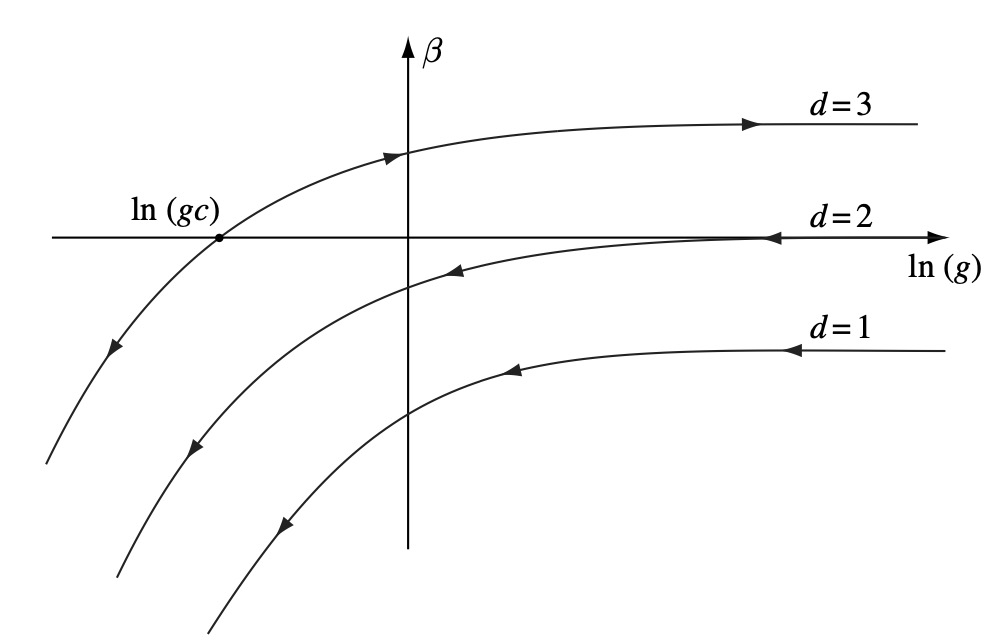
\includegraphics[width=0.4\linewidth]{pics/AL-RG-flow.jpg}
\end{equation*}
We see there is an order-disorder transition only at $d>2$.


\end{document}


